\section{The $W_q$ scale function and Discounting}
The underlying structure of ruin theory appears more clearly after generalizing the ruin problem to the two sided exit problem. Assume $a<b$, and consider quantities such as $\tau_a^+$, $\tau_b^-$, $\tau := \min\{ \tau_a^+, \tau_b^- \}$ and
\[ \Rui_{a,b}(x) = \mathbb{P}_x [\tau_a^+ < \tau_b^-] \]
\[ \sRui_{a,b}(x) = \mathbb{P}_x [\tau_a^+ > \tau_b^-]. \]

\begin{figure}
\caption{Sample path for a two sided exit problem}
\begin{center}
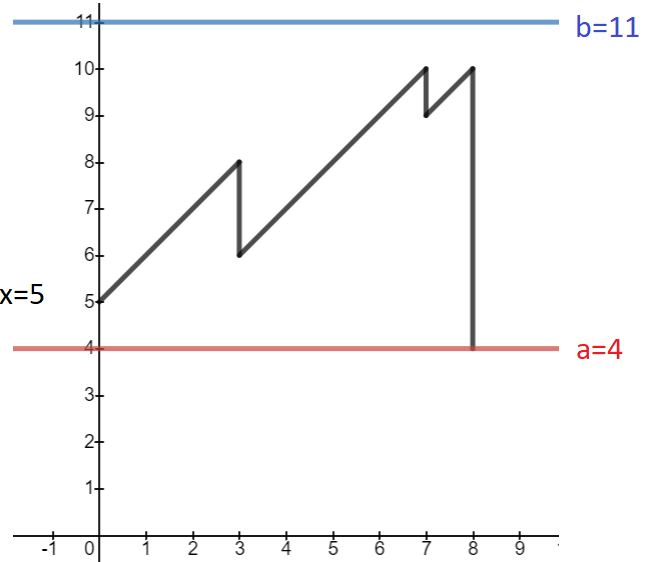
\includegraphics [width=2.3in]{twosided2.png}
\end{center}
\end{figure}

It can be shown, via the Markov property of the underlying process, that for some function $W$, we have
\[ \sRui_{a,b}(x) = \frac{W(x-a)}{W(b-a)}\]
We will refer to this function $W$ (determined up to a proportionality constant) as the $W$ scale function of the process.
Furthermore upon taking the Laplace transform of the previous equation we get
\[ \hat \sRui_{a,b}(s) = \frac{\hat W(s)}{W(b-a)}, \]
and in the case of the ruin problem where $\hat \sRui(s) = \frac{\kappa'(0)}{\kappa(s)}$, we get the idea that \[\hat W(s) = C \frac{1}{\kappa(s)}\] up to a certain constant $C$.

Generalizing further, suppose there exist an `interest rate' $q \geq 0$ such that one considers the `discounted value' of the underlying process with respect to this $q$ when deciding for the  first passage time.\\
In this scenario,
\[ \sRui_{a,b}(x) = \mathbb{E}_x [ e^{-q \tau_b^+} \cdot \mathbbm{1}_{\{\tau_a^+ > \tau_b^-\}}] \]
where $\mathbbm{1}_{A}$ is the event that $A$ happens.\\
Here the probability of survival considers all events where $\tau_a^+ > \tau_b^-$, and gets the expected value of the discounted value of 1 at the time $\tau_b^+$ with respect to $q$, hence the term $e^{-q \tau_b^+}$.

Even with discounting, through the same analysis as before one can find a function $W_q$ for which
\[ \sRui_{a,b}(x) = \frac{W_q(x-a)}{W_q(b-a)}. \]
In fact if one defines $W_q(s): (0,+\infty) \rightarrow [0,+\infty)$ to have a Laplace transform
\[ \hat{W}_q(s) = \int_0^{\infty} e^{-sx} W_q(x) ~dx  := \frac{1}{\kappa(s) - q} \quad \forall s > \Phi (q), \]
where $\Phi (q) := \sup \{ s\geq 0 : \kappa(s) - q = 0 \}$, one would arrive at such a function. As before we call this the $W_q$ scale function of the underlying process.\\

\begin{rmk} [\cite{Bingham}, \cite{Ber}, \cite{Kyp}]
The scale function $W_q$ is continuous and increasing on $[0,\infty]$.
\end{rmk}

\begin{rmk} [\cite{Kyprianou_Surya},\cite{KKP}]
The behavior in the neighborhood of zero of $W_q$ can be obtained from the behavior of its Laplace transform $\hat{W}_q$ at $\infty$
\begin{align}
\label{W0}
W_q (0^+) &= \lim_{s\rightarrow \infty} \frac{s}{\kappa(s)-q}= \begin{cases} \frac{1}{c} &\text{ if $X$ is of bdd variation}\\ 0 &
\text{ if $X$ is of unbdd variation} \end{cases}\\
\nonumber  W'_q (0^+) &= \lim_{s\rightarrow \infty} s\lt( \frac{s}{\kappa(s)-q} - W_q(0) \rt) \\
\label{Wprime0} &= \begin{cases} \frac{q + \nu (u,\infty)}{c^2} &\text{ if $X$ is of bdd variation}\\ \frac{2}{\sigma^2} & \text{ if $X$ is of unbdd variation} \end{cases}
\end{align}
\end{rmk}
